\documentclass[conference]{IEEEtran}
\IEEEoverridecommandlockouts

\usepackage{cite}
\usepackage{amsmath,amssymb}
\usepackage{graphicx}
\usepackage{booktabs}
\usepackage{url}
\usepackage[hidelinks]{hyperref}

\graphicspath{{../figuras/}}

% As tabelas e as figuras sao geradas pela execucao de homework2.ipynb.
% Nunca editar tabelas/*.tex na mao: rode o notebook de novo.

\begin{document}

% =====================================================================
% TITLE
% Alternativas consideradas (o enunciado pede que se tente mais de uma):
%   A) Regression Models for Aqueous Solubility: From Least Squares
%      Implemented from Scratch to a Neural Network          <- segura
%   B) Shrinkage Helps, Nonlinearity Helps More: Linear and Neural
%      Regression of the Aqueous Solubility of 1,267 Compounds
%   C) Why Linear Models Plateau on Aqueous Solubility: Evidence from
%      OLS, Ridge, PLS and a Neural Network          <- mais forte
% =====================================================================
\title{Shrinkage Helps, Nonlinearity Helps More: Linear and Neural
Network Regression of the Aqueous Solubility of 1{,}267 Compounds}

% Com 4 autores o \and do IEEEtran joga todos numa linha so e as colunas
% ficam com larguras diferentes, porque os nomes tem tamanhos diferentes.
% Duas linhas de dois, em minipages de largura fixa, ficam simetricas.
% Os macros \IEEEauthorblockN/A so funcionam na estrutura propria do \author
% do IEEEtran, entao dentro da minipage usamos formatacao direta, com os
% mesmos corpos de letra que eles aplicam.
\newcommand{\autorbloco}[2]{%
  \begin{minipage}[t]{0.46\textwidth}\centering
  {\normalsize #1}\\[0.35em]
  {\small #2\\
  \textit{Dep.\ de Eng.\ de Teleinformática}\\
  \textit{Universidade Federal do Ceará}}
  \end{minipage}}

% O \author do IEEEtran ja e um ambiente tabular, entao um \\ solto abriria
% linha nova nesse tabular e quebraria a compilacao. O \parbox isola.
\author{%
\parbox{\textwidth}{\centering
\autorbloco{Ícaro Adriano}{609310}\hfill\autorbloco{Matheus Reis}{571954}\\[1.4em]
\autorbloco{Alisson Jaime}{555083}\hfill\autorbloco{Vinícius A. G. do Nascimento}{568594}}
}

\maketitle

% =====================================================================
% ABSTRACT -- 4 frases: objetivo, dados, metodos, resultado.
% =====================================================================
\begin{abstract}
% [1] Objetivo
This work compares linear and nonlinear regression models for
predicting the aqueous solubility of chemical compounds from molecular
descriptors.
% [2] Dados
The dataset comprises $1{,}267$ compounds described by $228$ predictors,
208 binary structural fingerprints, 16 counts and 4 continuous
descriptors, split into $951$ training and $316$ test observations.
% [3] Metodos
After a Yeo-Johnson transformation that reduces the median absolute
skewness of the non-binary predictors from $1.36$ to $0.06$, we fit
ordinary least squares (OLS), ridge regression and partial least
squares (PLS), all implemented from scratch together with $10$-fold
cross-validation and checked against scikit-learn, and a single hidden
layer neural network, comparing them through repeated cross-validation
with corrected resampled $t$-tests.
% [4] Resultado principal
The three linear models are statistically indistinguishable on the test
set, with RMSE between $0.717$ and $0.743$ and $R^2$ between $0.872$ and
$0.881$, whereas the neural network reaches an RMSE of $0.620$ and an
$R^2$ of $0.911$, a difference significant against every linear model,
which indicates that part of the structure--solubility relationship is
nonlinear or interactive.
\end{abstract}

\begin{IEEEkeywords}
regression, ridge regression, partial least squares, neural networks,
cross-validation, aqueous solubility, QSPR
\end{IEEEkeywords}

% =====================================================================
% I. INTRODUCTION
% =====================================================================
\section{Introduction}
\label{sec:intro}

% --- P1: o que e regressao.
Regression is the task of learning, from $N$ observed pairs
$(\mathbf{x}_n, y_n)$, a function $f$ that predicts a continuous outcome
$y$ from a vector of $D$ predictors $\mathbf{x}$
\cite{hastie2009,kuhn2013}. The simplest and most interpretable choice
is a linear function fitted by ordinary least squares (OLS), which is
unbiased but becomes unstable when predictors are numerous and
collinear, because the variance of its coefficients grows with the
ill-conditioning of $\mathbf{X}^\top\mathbf{X}$.

% --- P2: familia de modelos.
Two families of remedies keep the model linear while trading a small
bias for a large reduction in variance. Penalised regression shrinks
the coefficients, either with an $L_2$ penalty (ridge regression
\cite{hoerl1970}) or with an $L_1$ penalty that also selects variables
(the lasso \cite{tibshirani1996}). Latent variable methods instead
regress the outcome on a few linear combinations of the predictors:
principal component regression (PCR) builds them from the predictors
alone, while partial least squares (PLS) builds them to covary with the
outcome \cite{wold2001}. When the relationship is not linear, a
multilayer perceptron with one hidden layer, trained by
back-propagation \cite{rumelhart1986}, can approximate any continuous
function given enough hidden units \cite{hornik1989}, at the price of a
non-convex fit and of a much larger number of parameters.

% --- P3: aplicacao: solubilidade/QSPR.
A classical application of these models is quantitative
structure--property relationship (QSPR) modelling in chemistry, and
aqueous solubility is one of its most studied targets, since a poorly
soluble compound is poorly absorbed and seldom becomes a drug.
Solubility has been predicted from topological indices with linear and
neural models \cite{huuskonen2000,tetko2001}, and simple linear
equations on a handful of descriptors such as ESOL remain a reference
in the field \cite{delaney2004}. The dataset used here is the
benchmark of Kuhn and Johnson \cite{kuhn2013}, derived from those
earlier compilations.

% --- P4: objetivo e organizacao.
This work fits and compares four regression models on that benchmark:
OLS, ridge regression, PLS and a neural network. The linear models and
the cross-validation are implemented from scratch and checked against
scikit-learn \cite{pedregosa2011}, and the comparison asks not only
which model has the lowest error but whether the differences are
statistically significant. Section~\ref{sec:methods} describes the data
and the methods, Section~\ref{sec:results} reports and discusses the
results, and Section~\ref{sec:conclusion} concludes.

% =====================================================================
% II. METHODS
% =====================================================================
\section{Methods}
\label{sec:methods}

\subsection{Dataset}
\label{subsec:dataset}

The dataset contains $N = 1{,}267$ compounds, provided already split
into $N_{tr} = 951$ training and $N_{ts} = 316$ test observations, and
$D = 228$ predictors with no missing values: 208 binary fingerprints
indicating the presence of a chemical substructure, 16 counts (atoms,
bonds, rings, halogens, etc.) and 4 continuous descriptors (molecular
weight, a hydrophilic factor and two surface areas)
\cite{kuhn2013}. The outcome is the base-10 logarithm of the
solubility, ranging from $-11.62$ to $1.58$ with mean $-2.72$ on the
training set and an almost identical distribution on the test set
(mean $-2.80$, standard deviation $2.08$ against $2.05$), so the
provided split is representative. The fingerprints are sparse but not
degenerate, with frequency of ones between $3.8\%$ and $86\%$.

\subsection{Pre-processing}
\label{subsec:preproc}

All 20 non-binary predictors are right-skewed, with skewness between
$0.67$ and $3.84$ (median $1.36$). To remove it we apply the
Yeo-Johnson transformation \cite{yeo2000}, a generalisation of the
Box-Cox family \cite{boxcox1964} that accepts zeros, which are common
among the counts, and negative values, present in the hydrophilic
factor:
\begin{equation}
\psi(x,\lambda)=
\begin{cases}
[(x+1)^{\lambda}-1]/\lambda, & x\ge 0,\ \lambda\neq 0,\\
-[(1-x)^{2-\lambda}-1]/(2-\lambda), & x<0,\ \lambda\neq 2,
\end{cases}
\label{eq:yj}
\end{equation}
with the logarithmic limits at $\lambda=0$ and $\lambda=2$. Each
$\lambda$ is estimated by maximum likelihood over $[-20, 20]$. Afterwards every
predictor, including the fingerprints, is standardised to zero mean and
unit variance. All parameters are estimated on the training set only
and applied unchanged to the test set; inside cross-validation they are
re-estimated in every fold from that fold's training part, so that the
held-out part never informs the pre-processing.

\begin{table}[htbp]
\caption{Yeo-Johnson parameter and skewness $\gamma$ before and after
the transformation for selected predictors (training set)}
\label{tab:skew}
\centering
\begin{tabular}{lrrrr}
\toprule
Predictor & $\hat\lambda$ & $\gamma$ raw & $\gamma$ transf. & Zeros \\
\midrule
MolWeight & 0.00 & 0.99 & -0.00 & 0\% \\
SurfaceArea1 & 0.35 & 1.71 & -0.23 & 23\% \\
HydrophilicFactor & -0.32 & 3.40 & 0.25 & 0\% \\
NumCarbon & 0.25 & 0.93 & -0.00 & 0\% \\
NumRotBonds & -0.08 & 1.58 & 0.02 & 29\% \\
NumOxygen & -0.17 & 1.77 & 0.04 & 34\% \\
NumChlorine & -3.63 & 3.18 & 1.42 & 79\% \\
NumSulfer & -9.77 & 3.84 & 2.24 & 87\%
\\
\bottomrule
\end{tabular}
\end{table}

\begin{figure}[htbp]
\centering
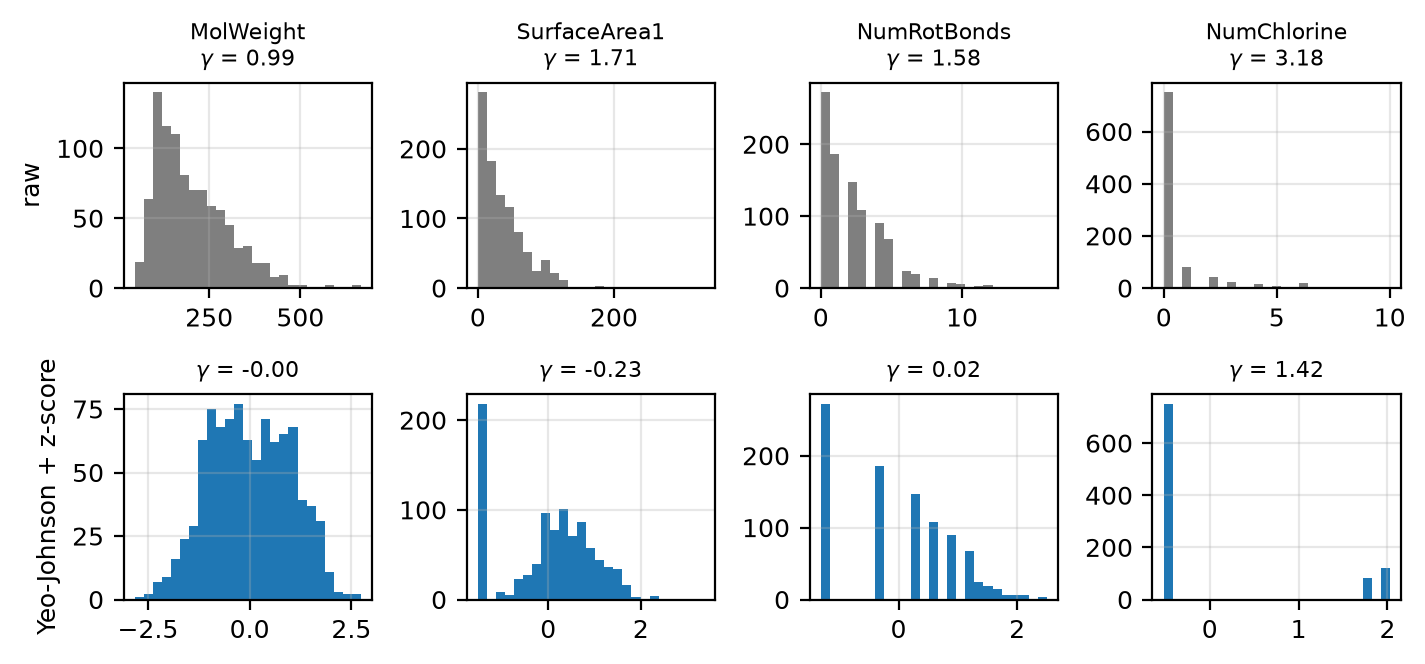
\includegraphics[width=\columnwidth]{assimetria_antes_depois.png}
\caption{Histograms of four predictors before (top) and after (bottom)
the Yeo-Johnson transformation and standardisation.}
\label{fig:skew}
\end{figure}

Table~\ref{tab:skew} and Fig.~\ref{fig:skew} show the effect. The
continuous descriptors and the counts with many distinct values become
practically symmetric, and the median absolute skewness of the 20
non-binary predictors drops from $1.36$ to $0.06$. The exceptions are
the counts dominated by zeros: sulfur, chlorine and halogen counts are
zero in $72\%$ to $87\%$ of the compounds and keep a skewness between
$1.0$ and $2.2$, because no monotonic transformation can spread a point
mass, only compress the tail (bottom right of Fig.~\ref{fig:skew}).

\subsection{Correlation structure}
\label{subsec:corr}

\begin{figure}[htbp]
\centering
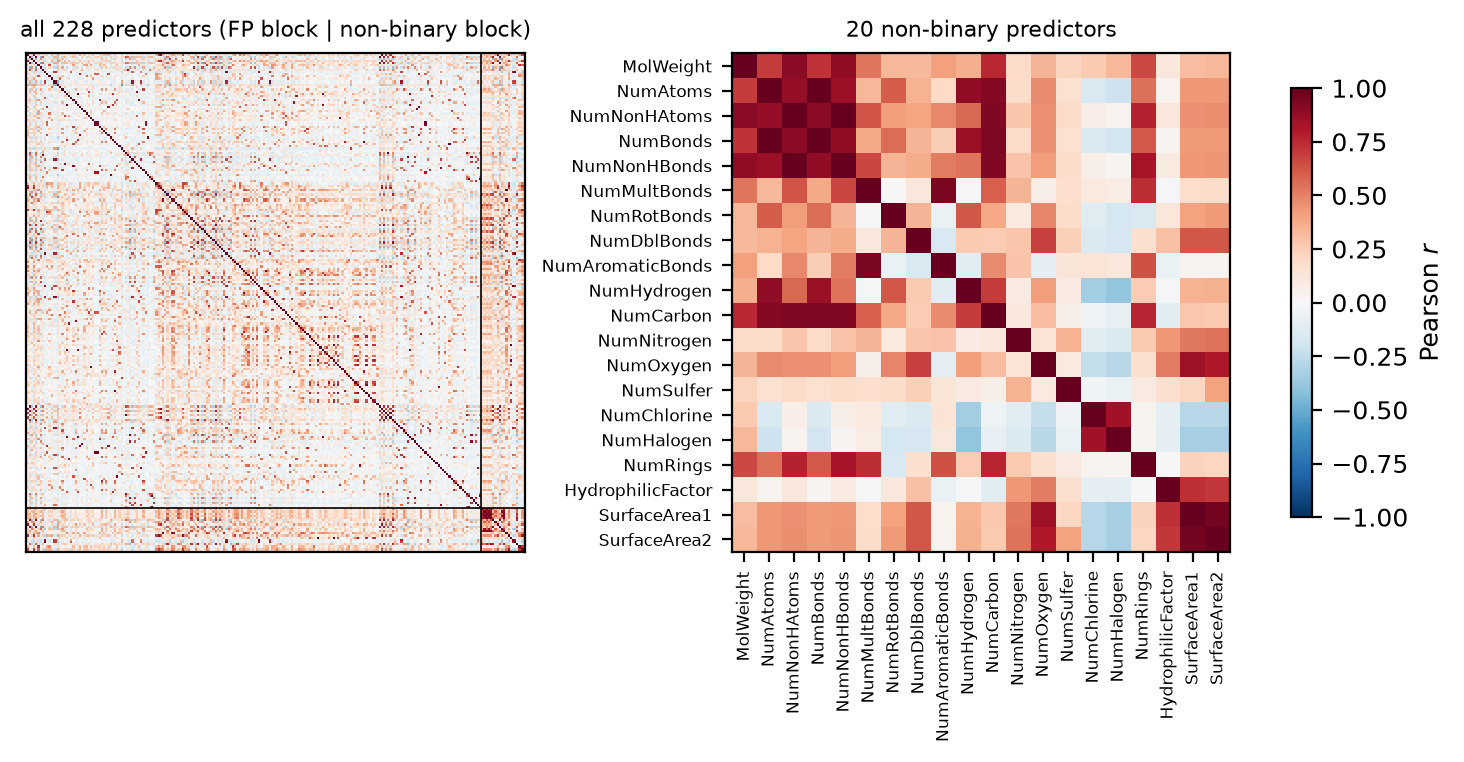
\includegraphics[width=\columnwidth]{matriz_correlacao.png}
\caption{Pearson correlation matrix of the transformed training
predictors: all 228 (left) and the 20 non-binary ones (right).}
\label{fig:corr}
\end{figure}

Fig.~\ref{fig:corr} shows the correlation matrix of the transformed
predictors. Among the $25{,}878$ pairs, the median absolute correlation
is only $0.091$, but $47$ pairs exceed $0.9$ and $7$ exceed $0.99$. The
strongest dependences are of two kinds. Size descriptors measure the
same property in different ways: number of atoms and of bonds
($r = 0.997$), of non-hydrogen atoms and bonds ($0.995$), and molecular
weight, carbon count and surface areas forming the dark block of the
right panel. And some fingerprints are near copies of a count, such as
FP134 and the sulfur count ($r = 1.000$) or FP107 and the chlorine
count ($0.999$). As a consequence the eigenvalues of the correlation
matrix range from $28.3$ down to $2.9\times10^{-8}$, a condition number
of $10^{9}$, and $22$ eigenvalues are below $0.01$. This is the
regime in which OLS coefficients are unstable and shrinkage or latent
variable methods should help.

\begin{figure}[htbp]
\centering
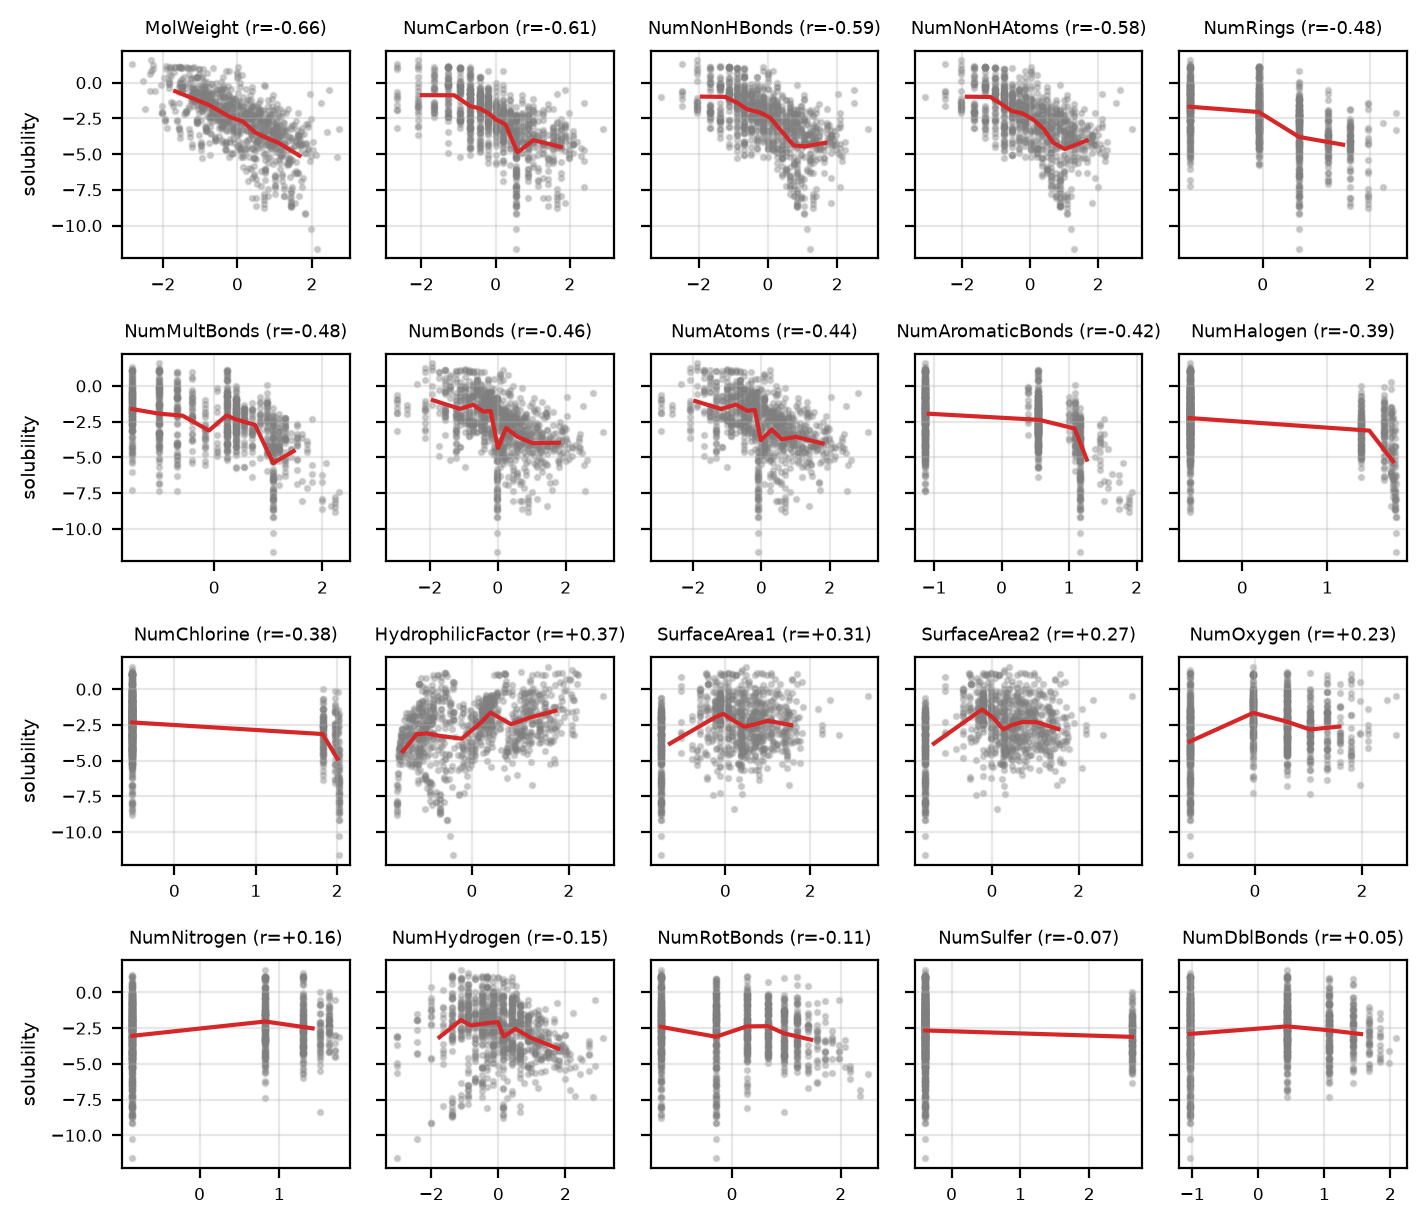
\includegraphics[width=\columnwidth]{preditores_vs_desfecho.png}
\caption{Solubility against each transformed non-binary predictor,
sorted by $|r|$, with the mean outcome in deciles of the predictor
(red).}
\label{fig:yx}
\end{figure}

Fig.~\ref{fig:yx} relates each non-binary predictor to the outcome. The
strongest individual correlations are all negative and all measure
molecular size: molecular weight ($r=-0.66$), carbon count ($-0.61$)
and non-hydrogen bonds and atoms ($-0.58$), which agrees with the
chemical intuition that larger molecules are less soluble in water.
Only six predictors have $|r| > 0.5$ and the median $|r|$ over all 228
is $0.096$; the strongest fingerprint, FP076, reaches $r = -0.54$. To
judge linearity quantitatively we compared, for each non-binary
predictor, the $R^2$ of a univariate straight line with that of a cubic
polynomial. The gain is below $0.05$ for 12 of the 20 predictors, so
after the transformation most individual relations are close to linear.
The largest gains, up to $0.13$, occur for the aromatic bond count, the
surface areas and the halogen counts, all with a large share of zeros,
where the red curves in Fig.~\ref{fig:yx} change slope between the
zero and the positive values. For the fingerprints linearity holds
trivially, since a binary predictor takes only two values.

\subsection{Regression models}
\label{subsec:models}

\emph{OLS.} With the design matrix $\mathbf{A}=[\mathbf{1}\ \mathbf{Z}]$
of the transformed predictors, the coefficients solve the normal
equations
\begin{equation}
\hat{\boldsymbol\beta}_{\mathrm{OLS}} =
(\mathbf{A}^\top\mathbf{A})^{-1}\mathbf{A}^\top\mathbf{y}.
\label{eq:ols}
\end{equation}
We solve the linear system directly and, when $\mathbf{A}$ is rank
deficient, fall back to the minimum-norm solution
$\mathbf{A}^{+}\mathbf{y}$ given by the Moore-Penrose pseudo-inverse.
OLS is unbiased, has no tuning parameter and is fully interpretable,
but with $229$ coefficients and the collinearity above its variance is
high.

\emph{Ridge regression} adds an $L_2$ penalty on the slopes, leaving
the intercept free. With centred $\mathbf{Z}_c$ and $\mathbf{y}_c$,
\begin{equation}
\hat{\boldsymbol\beta}_{\lambda} =
(\mathbf{Z}_c^\top\mathbf{Z}_c + \lambda\mathbf{I})^{-1}
\mathbf{Z}_c^\top\mathbf{y}_c .
\label{eq:ridge}
\end{equation}
Adding $\lambda$ to every eigenvalue of $\mathbf{Z}_c^\top\mathbf{Z}_c$
removes the ill-conditioning and shrinks the coefficients toward zero
\cite{hoerl1970}. Its cost is a bias that grows with $\lambda$, which
must be tuned, and, unlike the lasso, it never sets a coefficient
exactly to zero.

\emph{PLS} regresses $y$ on $A \ll D$ latent scores
$\mathbf{t}_a = \mathbf{E}_{a-1}\mathbf{w}_a$, where the weight vector
$\mathbf{w}_a \propto \mathbf{E}_{a-1}^\top\mathbf{f}_{a-1}$ maximises
the covariance between the deflated predictors $\mathbf{E}$ and the
deflated outcome $\mathbf{f}$ \cite{wold2001}. We implemented the
NIPALS algorithm for a single outcome, whose coefficients in the
original space are
$\boldsymbol\beta = \mathbf{W}(\mathbf{P}^\top\mathbf{W})^{-1}\mathbf{q}$,
with $\mathbf{P}$ the predictor loadings and $\mathbf{q}$ the outcome
loadings. PLS was preferred to PCR because its components are guided
by the outcome, so it usually needs fewer of them; its drawbacks are
the tuning of $A$ and components that are harder to interpret than
principal components.

\emph{Neural network.} We use a multilayer perceptron with one hidden
layer of $H$ hyperbolic tangent units and a linear output,
\begin{equation}
\hat y = b + \sum_{h=1}^{H} v_h \tanh\!\left(c_h + \mathbf{u}_h^\top\mathbf{z}\right),
\label{eq:mlp}
\end{equation}
trained with L-BFGS on the squared error plus a weight decay
$\alpha\lVert\mathbf{w}\rVert^2$, using scikit-learn
\cite{pedregosa2011}, with the outcome standardised during training.
The network can represent curvature and interactions that the linear
models cannot \cite{hornik1989}, but it has $H(D+2)+1$ parameters, over
$9{,}000$ for $H = 40$, its fit is non-convex and depends on the random
initialisation, and it is far less interpretable.

\subsection{Model assessment}
\label{subsec:assess}

Performance is measured by
$\mathrm{RMSE} = \sqrt{\frac{1}{N}\sum_n (y_n-\hat y_n)^2}$ and by
$R^2 = 1 - \sum_n (y_n-\hat y_n)^2 / \sum_n (y_n-\bar y)^2$. The
$K$-fold cross-validation (CV) was implemented from scratch: the
training indices are shuffled with a fixed seed and split into $K=10$
folds, and every model and hyper-parameter is evaluated on the same
partitions. Hyper-parameters are chosen by the minimum mean CV RMSE
using the training set only: $\lambda$ among 30 values log-spaced in
$[10^{-2},10^{4}]$, $A$ from 1 to 40, and $(H,\alpha)$ in
$\{5,10,20,40\}\times\{1,3,10,30,100\}$. The test set is used once, for
the final models, with $95\%$ bootstrap confidence intervals for the
RMSE ($2{,}000$ resamples).

To decide whether two models differ, we repeat the 10-fold CV five
times with new partitions and fixed hyper-parameters and apply to the
50 paired differences of RMSE the corrected resampled $t$-test of
Nadeau and Bengio \cite{nadeau2003},
\begin{equation}
t = \frac{\bar d}{\sqrt{\left(\frac{1}{J}+\frac{N_{va}}{N_{tr}}\right)s_d^2}},
\label{eq:nb}
\end{equation}
with $J=50$ and $J-1$ degrees of freedom; the term
$N_{va}/N_{tr}$ corrects the optimism of the ordinary paired $t$-test,
whose samples are not independent because the training sets overlap.
On the test set we apply the Wilcoxon signed-rank test
\cite{wilcoxon1945} to the paired squared errors of each compound. In
both cases the $p$-values of the six pairs are adjusted with Holm's
procedure \cite{holm1979}.

% =====================================================================
% III. RESULTS
% =====================================================================
\section{Results and Discussion}
\label{sec:results}

\subsection{Ordinary least squares}
\label{subsec:res_ols}

\begin{table}[htbp]
\caption{OLS: implementation from scratch against scikit-learn, and
test set against cross-validation estimates (mean $\pm$ standard
deviation over folds)}
\label{tab:ols}
\centering
\begin{tabular}{lll}
\toprule
Estimate & RMSE & $R^2$ \\
\midrule
Test set, from scratch & 0.7430 & 0.8718 \\
Test set, scikit-learn & 0.7430 & 0.8718 \\
\midrule
10-fold CV, from scratch & 0.7279 $\pm$ 0.068 & 0.8654 $\pm$ 0.040 \\
10-fold CV, scikit-learn & 0.7279 $\pm$ 0.068 & 0.8654 $\pm$ 0.040 \\
5-fold CV, from scratch & 0.7705 $\pm$ 0.060 & 0.8513 $\pm$ 0.046
\\
\bottomrule
\end{tabular}
\end{table}

Table~\ref{tab:ols} summarises the OLS model. The implementation from
scratch and scikit-learn give the same test RMSE of $0.743$ and $R^2$
of $0.872$, with predictions equal to $10^{-8}$; the coefficients agree
only to $5\times10^{-6}$, which is what a condition number of $10^{9}$
allows. The two cross-validations agree fold by fold to $10^{-7}$. The full training matrix has
full rank, but two of the ten folds do not: when part of the compounds
is held out, some rare fingerprints become exact copies of another
predictor, and there the pseudo-inverse branch of \eqref{eq:ols} is
required, a failure mode that a naive solution of the normal equations
turns into predictions of order $10^{12}$. The training RMSE of $0.49$
against a test RMSE of $0.74$ shows the overfitting expected from 229
coefficients. The 10-fold estimate, $0.728 \pm 0.068$, slightly
underestimates the test error, and the 5-fold estimate, $0.771 \pm
0.060$, slightly overestimates it, as expected since each 5-fold model
is trained on only $80\%$ of the data. The test RMSE lies between the
two and within one standard deviation of both; with only $316$ test
compounds it carries itself an uncertainty of about $\pm0.08$
(Table~\ref{tab:results}), so CV and test set are consistent.

\subsection{Ridge regression}
\label{subsec:res_ridge}

\begin{figure}[htbp]
\centering
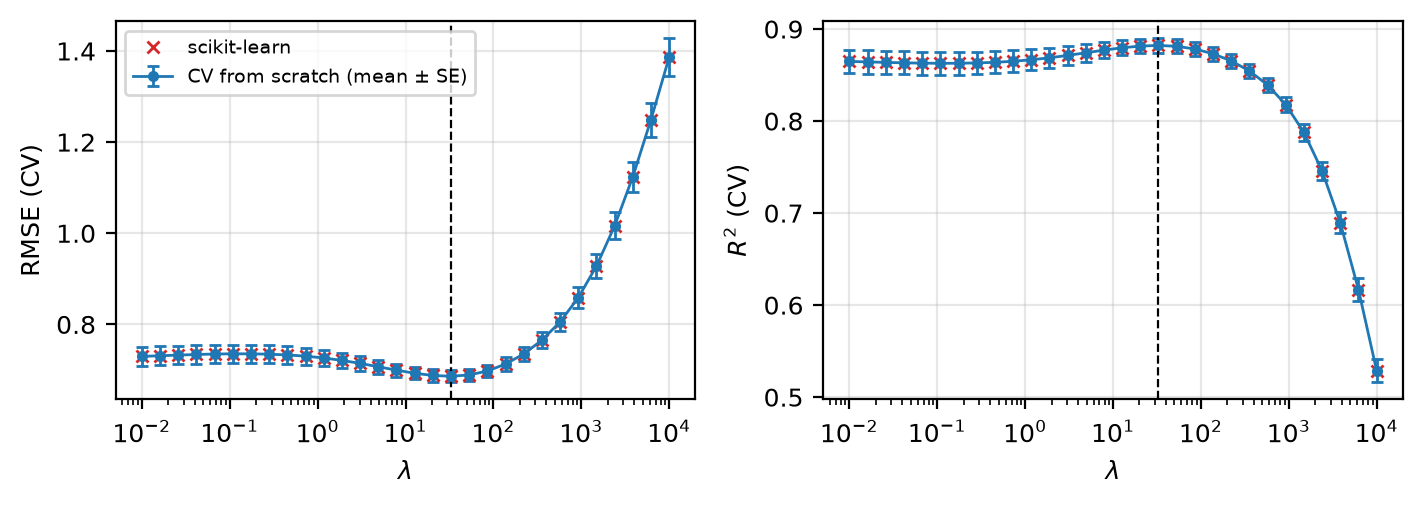
\includegraphics[width=\columnwidth]{perfil_cv_ridge.png}
\caption{Ridge: 10-fold CV profile of RMSE (left) and $R^2$ (right)
against $\lambda$, mean $\pm$ standard error over folds; red crosses
are scikit-learn's \texttt{GridSearchCV}. The dashed line marks the
selected $\lambda$.}
\label{fig:ridge}
\end{figure}

Fig.~\ref{fig:ridge} shows the CV profile. For small $\lambda$ ridge
coincides with OLS; the RMSE then decreases to a minimum of $0.686$ at
$\lambda = 32.9$, where the CV $R^2$ is $0.882$, and grows quickly once
the penalty shrinks the coefficients too much, reaching $1.39$ at
$\lambda = 10^4$. The profile computed by scikit-learn on the same
folds overlaps ours to within $10^{-8}$ and selects the same $\lambda$,
and for a fixed $\lambda$ the two coefficient vectors agree to
$5\times10^{-14}$. At the selected value the norm of the coefficient
vector drops from $152$ (OLS) to $1.5$, and the test RMSE improves from
$0.743$ to $0.717$ ($R^2 = 0.881$). The one-standard-error rule would
choose the more regularised $\lambda = 85$ at almost the same CV error.

\subsection{Partial least squares}
\label{subsec:res_pls}

\begin{figure}[htbp]
\centering
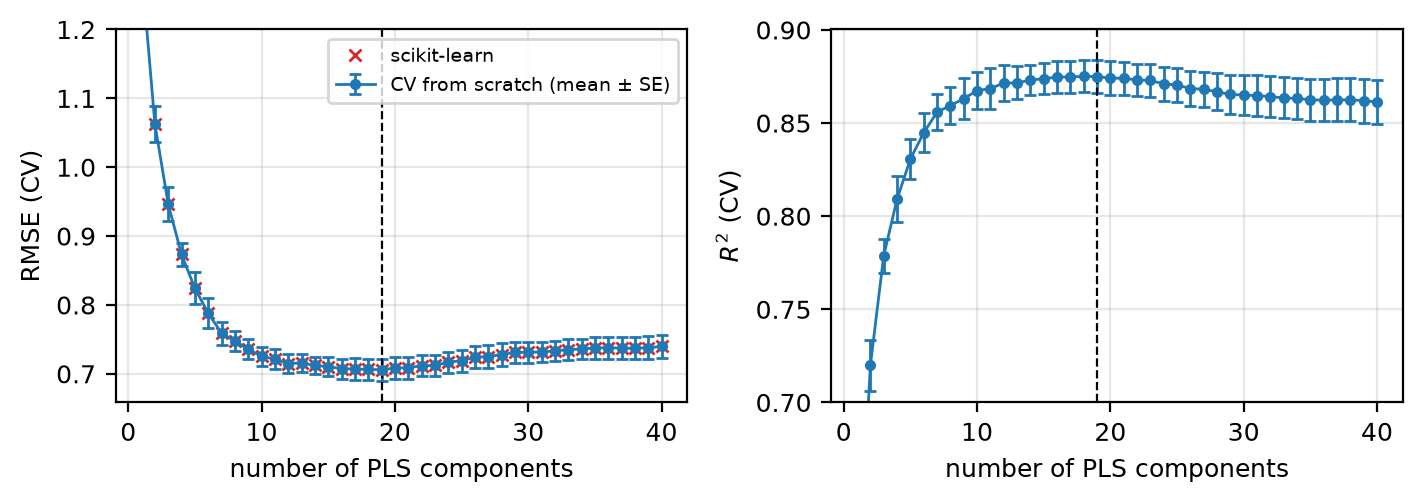
\includegraphics[width=\columnwidth]{perfil_cv_pls.png}
\caption{PLS: 10-fold CV profile of RMSE (left) and $R^2$ (right)
against the number of components; red crosses are scikit-learn's
\texttt{PLSRegression}. The dashed line marks the selected value.}
\label{fig:pls}
\end{figure}

Our NIPALS implementation matches scikit-learn's \texttt{PLSRegression}
to $2\times10^{-15}$ in the coefficients. Fig.~\ref{fig:pls} shows that
the CV RMSE falls steeply over the first ten components, from $1.29$
with one component to $0.73$ with ten, reaches its minimum of $0.706$
($R^2 = 0.875$) at $A = 19$ and then slowly rises toward the OLS value
as more components are added. With fewer than a tenth of the 228
dimensions PLS already matches OLS, confirming that the information on
solubility is concentrated in a few latent directions. On the test set
the 19-component model reaches an RMSE of $0.734$ and an $R^2$ of
$0.875$. The one-standard-error rule would select only $11$ components.

\subsection{Neural network}
\label{subsec:res_mlp}

\begin{figure}[htbp]
\centering
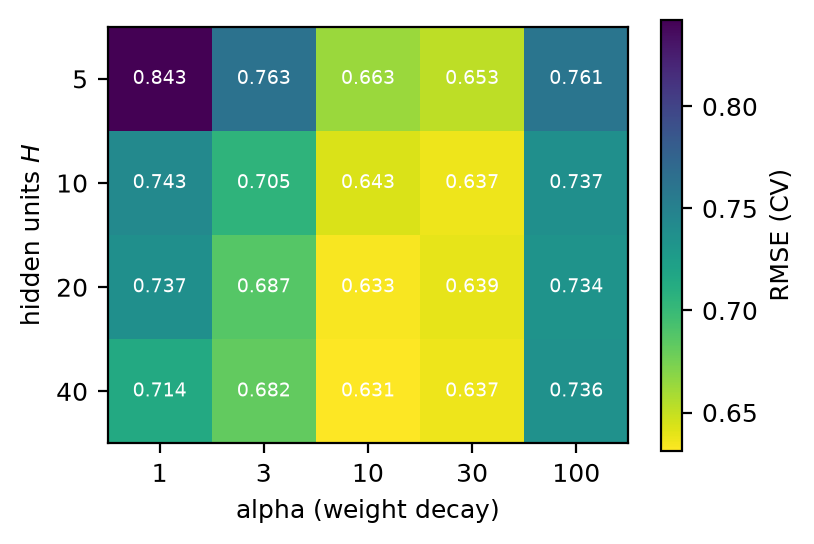
\includegraphics[width=0.8\columnwidth]{grade_cv_mlp.png}
\caption{Neural network: 10-fold CV RMSE over the grid of hidden units
$H$ and weight decay $\alpha$.}
\label{fig:mlp}
\end{figure}

Fig.~\ref{fig:mlp} shows the CV RMSE over the hyper-parameter grid.
Weight decay is decisive: with $\alpha = 1$ even large networks overfit
(CV RMSE above $0.70$), whereas $\alpha$ between $10$ and $30$ gives the
best results for every $H$, and $\alpha = 100$ underfits. With adequate
regularisation the error decreases with $H$ and flattens beyond
$H = 20$, the best configuration being $H = 40$, $\alpha = 10$, with a
CV RMSE of $0.631$ and $R^2$ of $0.900$. On the test set it reaches an
RMSE of $0.620$ and an $R^2$ of $0.911$. Retraining with ten random
initialisations gives a test RMSE of $0.631 \pm 0.010$, so the result
does not depend on a fortunate seed.

\subsection{Model comparison}
\label{subsec:res_comp}

\begin{table*}[htbp]
\caption{Performance of the four models: 10-fold CV on the training set
and test set, with $95\%$ bootstrap confidence interval for the test
RMSE}
\label{tab:results}
\centering
\begin{tabular}{llrrrcr}
\toprule
Model & Hyper-parameter & RMSE (CV) & $R^2$ (CV) & RMSE (test) & 95\% CI & $R^2$ (test) \\
\midrule
OLS & --- & 0.728 & 0.865 & 0.743 & 0.668--0.822 & 0.872 \\
Ridge & $\lambda = 32.9$ & 0.686 & 0.882 & 0.717 & 0.646--0.791 & 0.881 \\
PLS & $A = 19$ & 0.706 & 0.875 & 0.734 & 0.663--0.806 & 0.875 \\
MLP & $H = 40$, $\alpha = 10$ & 0.631 & 0.900 & 0.620 & 0.549--0.694 & 0.911
\\
\bottomrule
\end{tabular}
\end{table*}

\begin{figure}[htbp]
\centering
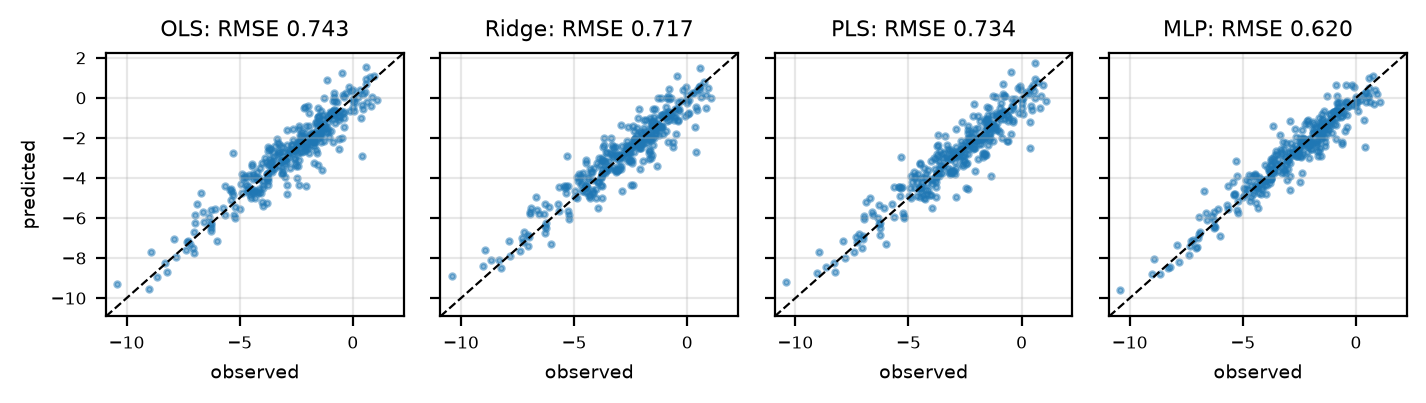
\includegraphics[width=\columnwidth]{observado_vs_predito.png}
\caption{Observed against predicted solubility on the test set.}
\label{fig:obspred}
\end{figure}

\begin{figure}[htbp]
\centering
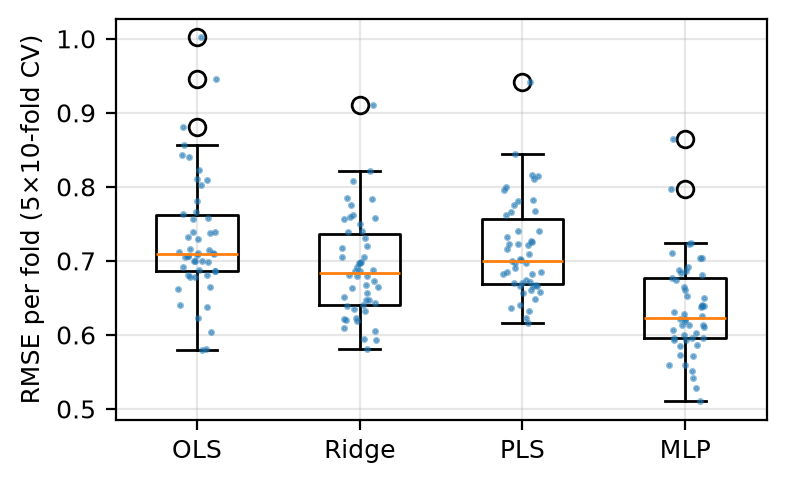
\includegraphics[width=0.8\columnwidth]{cv_repetida_modelos.png}
\caption{RMSE per fold over five repetitions of 10-fold CV, with the
hyper-parameters fixed at the selected values.}
\label{fig:cvrep}
\end{figure}

\begin{table}[htbp]
\caption{Pairwise comparisons: mean RMSE difference (first minus
second model) and Holm-adjusted $p$-values of the corrected resampled
$t$-test (repeated CV) and of the Wilcoxon test (test set)}
\label{tab:tests}
\centering
\begin{tabular}{lrrrr}
\toprule
& \multicolumn{2}{c}{Repeated CV} & \multicolumn{2}{c}{Test set} \\
Pair & $\Delta$RMSE & $p$ & $\Delta$RMSE & $p$ \\
\midrule
OLS vs. Ridge & +0.039 & 0.081 & +0.026 & 0.872 \\
OLS vs. PLS & +0.014 & 0.386 & +0.009 & 0.872 \\
OLS vs. MLP & +0.095 & $<0.001$ & +0.123 & $<0.001$ \\
Ridge vs. PLS & -0.024 & 0.008 & -0.016 & 0.205 \\
Ridge vs. MLP & +0.056 & $<0.001$ & +0.097 & $<0.001$ \\
PLS vs. MLP & +0.080 & $<0.001$ & +0.114 & $<0.001$
\\
\bottomrule
\end{tabular}
\end{table}

Table~\ref{tab:results} collects the results. The three linear models
form a tight group, with test RMSE from $0.717$ to $0.743$ and $R^2$
from $0.872$ to $0.881$, and their confidence intervals overlap almost
entirely. The neural network stands apart with a test RMSE of $0.620$,
$14\%$ to $17\%$ lower, and an $R^2$ of $0.911$. Fig.~\ref{fig:obspred}
shows that all four models share the same pattern of shrinkage toward
the mean: splitting the test compounds by solubility, the mean error
(observed minus predicted) is between $-0.19$ and $-0.43$ for the 29
compounds below $-6$, which are predicted too soluble, and between
$+0.53$ and $+0.60$ for the 20 above $0$. The network does not remove
this pattern, but it has the lowest RMSE in every one of the five
ranges of solubility examined, so its gain is spread over the whole
outcome range rather than confined to a few extreme compounds.

Fig.~\ref{fig:cvrep} and Table~\ref{tab:tests} answer whether the
differences are statistically significant. Among the linear models,
neither OLS against ridge ($p = 0.081$ in CV) nor OLS against PLS is
significant on either test, and ridge against PLS is significant in the
repeated CV ($p = 0.008$) but not on the test set ($p = 0.21$): the advantage of
ridge is consistent across folds but too small, $0.02$ in RMSE, to be
detected on 316 compounds. The neural network, in contrast, is better
than every linear model with Holm-adjusted $p$-values below $0.001$ on
both tests. The standard deviation of the RMSE between folds, $0.07$
to $0.08$, is larger than the differences among the linear models,
which is why a single split is not enough to rank them.

The nonlinear model therefore outperforms the linear ones, and the
improvement is not an artefact of a particular partition or seed. This
says that the relationship between the descriptors and solubility is
not fully captured by an additive linear function, even after the
transformation that made most individual relations nearly linear
(Section~\ref{subsec:corr}). Since the gain is spread over all ranges of the outcome,
the remaining structure is most likely in interactions between
predictors, such as the effect of a substructure depending on the size
of the molecule, and in the residual curvature of the zero-inflated
counts noted in Section~\ref{subsec:corr}; a linear model can only
represent these if they are engineered explicitly as new features. Shrinkage and latent components tame the
variance of the linear fit, but they cannot add the missing nonlinear
terms, which explains why ridge and PLS improve on OLS only marginally
while the network improves on all of them.

% =====================================================================
% IV. CONCLUSION
% =====================================================================
\section{Conclusion}
\label{sec:conclusion}

We fitted four regression models to the aqueous solubility of $1{,}267$
compounds. The Yeo-Johnson transformation removed most of the skewness
of the descriptors, and the exploratory analysis revealed strong
collinearity among size descriptors and between fingerprints and
counts, with a condition number of $10^{9}$. The
implementations from scratch of OLS, ridge regression, PLS and
cross-validation reproduced scikit-learn to numerical precision, once
rank-deficient folds were handled with the pseudo-inverse. Ridge and
PLS controlled the variance caused by collinearity and improved
slightly on OLS, but the three linear models remained statistically
indistinguishable on the test set, with RMSE around $0.72$--$0.74$. A
single hidden layer neural network lowered the test RMSE to $0.62$ and
raised $R^2$ to $0.91$, a significant improvement under both the
corrected resampled $t$-test and the Wilcoxon test, which indicates
that part of the structure--solubility relationship is nonlinear or
interactive. Natural extensions are nonlinear models that remain
interpretable, such as tree ensembles, and nested cross-validation, so
that the hyper-parameter search is also accounted for in the
comparison.

% =====================================================================
% Declaracao de uso de IA. O enunciado permite que os prompts e as
% respostas fiquem num arquivo separado do repositorio, e e la que
% estao, para nao ocupar as 6 paginas do artigo.
\section*{Use of AI Tools}
AI assistance (Anthropic Claude) was used in this work. The prompts,
the responses and the use made of each are recorded in
\texttt{USO\_DE\_IA.md} in the project repository.

% =====================================================================
% REFERENCES
% =====================================================================
\bibliographystyle{IEEEtran}
\bibliography{refs}

\end{document}
